\section{Methodology}
\label{sec:method}

Our system has four components: (1) feature engineering, (2) a dual-path neural network with cross-modal gating, (3) gradient-boosted tree models, and (4) a weighted probability ensemble.

\begin{figure}[H]
\centering
% FIGURE: System Overview — REGENERATE NEEDED (update weights and OOF)
% Generate: figures/system_overview.png
%
% Layout: Left-to-right flow, 3 columns:
%
% Column 1 (Data Sources) — 3 rounded boxes stacked:
%   "Radiology Report" (blue border)
%   "Clinical + SI + Location" (green border)
%   "Image Features (PCA)" (gray border, label "inactive in NN" in small text)
%
% Column 2 (Models) — 3 rounded boxes:
%   "Neural Network" with subtitle "BERT + Tabular + CrossModalGate"
%   "MLU Models" with subtitle "XGB + LGB + CB"
%   "Auxiliary" with subtitle "NNXGB (NN probs→XGB) + ImgTab"
%
% Column 3 (Ensemble) — 1 box:
%   "Weighted Blend" with subtitle "87.25% OOF"
%
% Arrows:
%   Report → Neural Network (blue)
%   Report → MLU Models (blue)
%   Clinical+SI+Location → Neural Network (green)
%   Clinical+SI+Location → MLU Models (green)
%   Clinical+SI+Location → Auxiliary (green)
%   Image → Auxiliary (gray, dashed)
%   All 3 model boxes → "Weighted Blend"
%
% Below "Weighted Blend" box, show weights (submission config):
%   NN: 40%  |  MLU_XGB: 30%  |  MLU_LGB: 30%  |  MLU_CB: 0%  |  NNXGB: 5%  |  ImgTab: 5%  (grid-search optimal)
%
% Style: Clean, white background, rounded corners, no internal details.
% Figure size: (12, 5), tight layout
%
% Data source: model_final.ipynb Cell 25
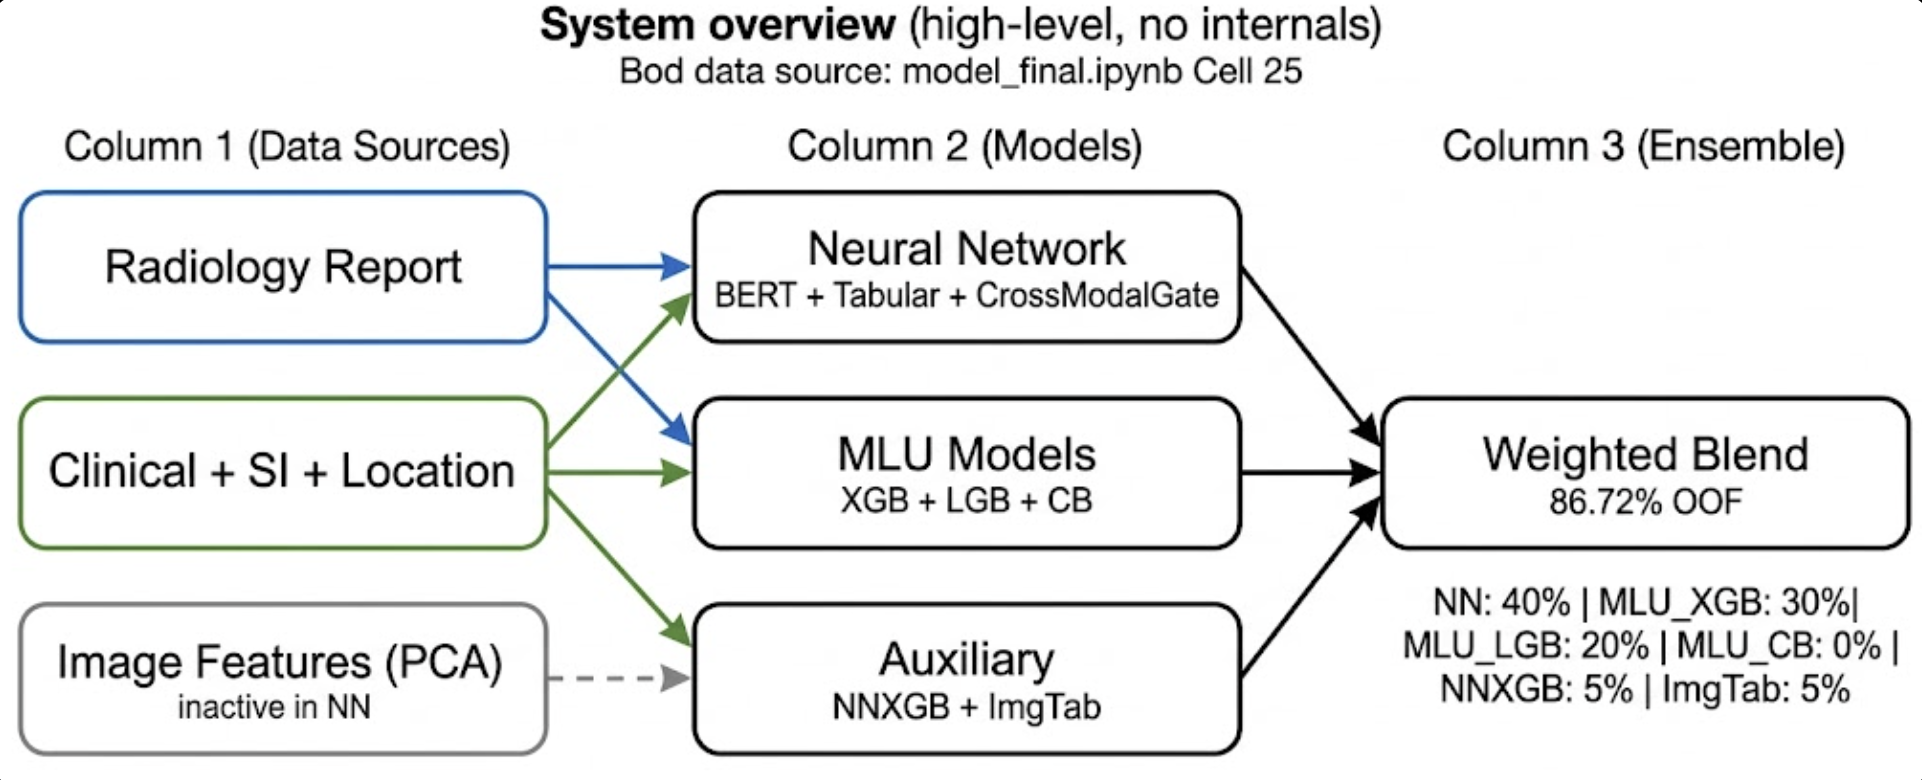
\includegraphics[width=\textwidth]{figures/system_overview.png}
\caption{System overview. Radiology reports and clinical features feed into both neural network and tree models. NNXGB uses the NN's 5-d class probabilities as input features for XGBoost. The image path is used only in the ImgTab auxiliary model (dashed arrow). All 6 model probabilities are combined via weighted blend achieving 87.25\% OOF Micro-F1.}
\label{fig:system_overview}
\end{figure}

\subsection{Feature Engineering}
\label{sec:feat_eng}

Our preprocessing mirrors how radiologists read scans: they compare across MRI sequences, combine findings with anatomical location, and consider patient demographics. Table~\ref{tab:feature_summary} summarizes all features.

\begin{table}[H]
\centering
\caption{Summary of engineered features.}
\label{tab:feature_summary}
\begin{tabular}{llcl}
\toprule
\textbf{Source} & \textbf{Encoding} & \textbf{Dim} & \textbf{Used By} \\
\midrule
Report (TF-IDF+SVD) & Trigram TF-IDF $\to$ SVD-256 & 256 & MLU tree models \\
Report (BERT) & BioClinicalBERT CLS token & 768 & Neural network \\
Demographics & Sex, Age, Age\_missing & 3 & NN tabular + ImgTab \\
Signal Intensity & One-hot, 6 values $\times$ 4 modalities & 24 & NN tabular + ImgTab \\
Location (label) & Learned embedding & 10 & NN tabular \\
Location (hierarchy) & Region + hemisphere + lobe & 3 & NN tabular + MLU \\
Cross-modal Ratios & Log ratios across modalities & 25 & NN tabular + MLU \\
Missing flags & Per-modality radiomics & 4 & NN tabular \\
SI Unknown ratio & Fraction of unknown SI & 1 & MLU \\
Image (PCA) & Per-modality PCA & 512 & ImgTab \\
\bottomrule
\end{tabular}
\end{table}

\textbf{Key design choices:}

\begin{itemize}
  \item \textbf{Location has two representations:} A label-encoded index (for the NN embedding) and a hierarchical parse into region/hemisphere/lobe (3 features). The hierarchy handles novel test locations---even if ``left posterior frontal gyrus'' is unseen, we extract region=brain, hemisphere=left, lobe=frontal.
  \item \textbf{Cross-modal ratios:} We compute T1c/T1 (enhancement), T2F/T2 (edema), T1/T2 (tissue contrast), and their deltas for each of 5 radiomic features (25 total). These transform absolute texture statistics into clinically meaningful relative contrasts. However, experiments show these ratios alone remain near-random ($\sim$52\%); we include them as they encode domain knowledge at zero cost.
  \item \textbf{Per-modality PCA for images:} Mean-pooling destroys complementary physical information (T1/T1c = anatomy/vascularity; T2/T2F = edema). Per-modality PCA (128d each, 94.16\% variance explained) preserves each sequence's diagnostic signal.
\end{itemize}

\subsection{Dual-Path Neural Network}
\label{sec:nn}

\textbf{Why dual-path, not unified transformer?} Our initial architecture (v1) used a 6-token transformer giving equal weight to all modalities. It failed ($\sim$80\%) because weak modalities (image $\sim$57\%, radiomics $\sim$52\%) dragged down the strong ones (report $\sim$84\%). The dual-path design isolates each modality's encoding so weak features cannot contaminate strong ones.

\subsubsection{Report Encoder}

\begin{figure}[H]
\centering
% FIGURE: Report Encoder Detail
% Generate: figures/report_encoder.png
%
% Layout: Vertical flow diagram
%
% [Input: Token IDs, shape (128,)]  ← show as small box
%          ↓
% [BioClinicalBERT]  ← large box, split into two sections:
%   Top section: "Layers 0–9 (frozen)" — gray background, padlock icon
%   Bottom section: "Layers 10–11 (fine-tuned)" — blue background
%          ↓
% [CLS token, 768d]  ← small box
%          ↓ fork into two branches side by side:
%
%   Left branch:                    Right branch:
%   [Linear 768→288]               [Linear 768→288]
%   [LayerNorm → GELU]             (no activation, just linear)
%   [Dropout 0.15]
%        ↓                              ↓
%   proj_out (288d)               residual (288d)
%        ↓────────── + ──────────────↓
%                   ↓
%             report_emb (288d)
%
% Annotations:
%   - Mark "768d" and "288d" on arrows
%   - Label the sum node as "residual connection"
%   - Show "Dropout 0.15" only on left branch
%
% Figure size: (10, 6), clean style
%
% Data source: model_final.ipynb Cell 14
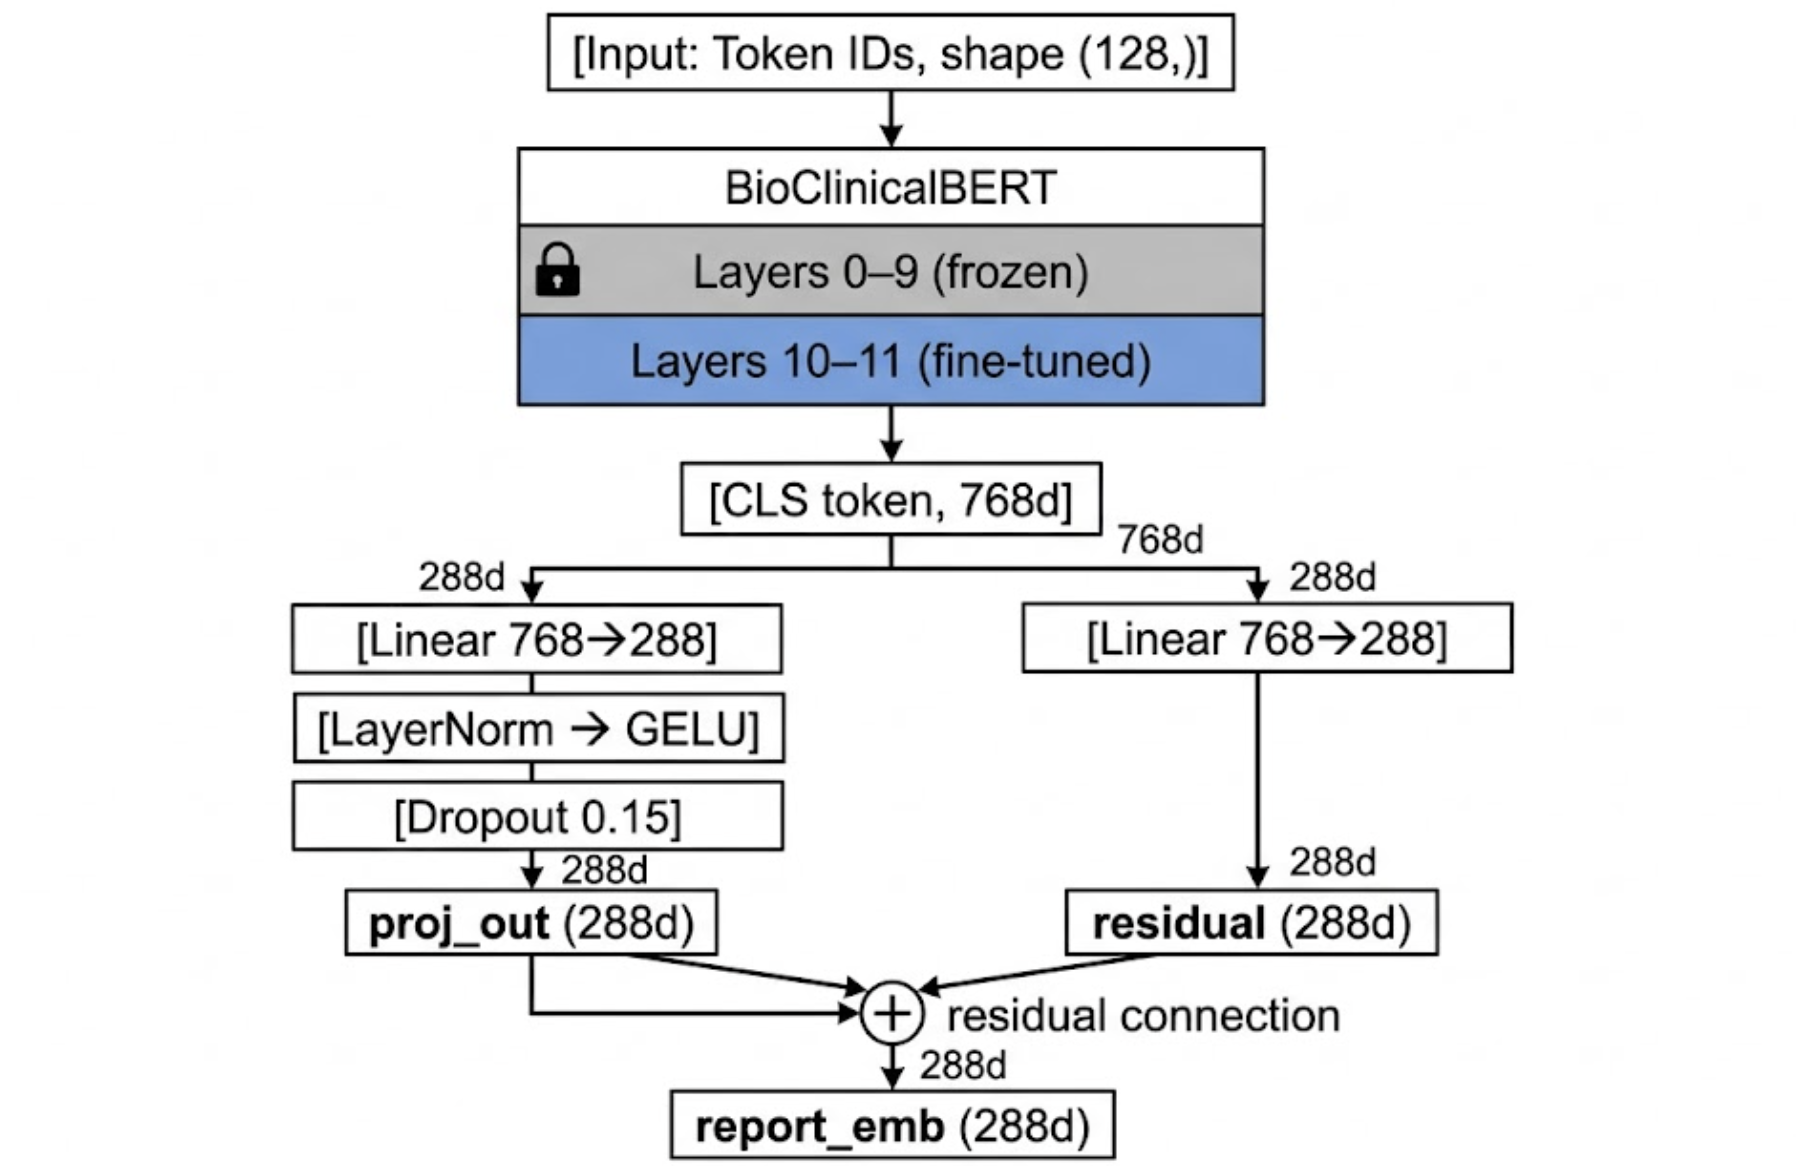
\includegraphics[width=0.75\textwidth]{figures/report_encoder.png}
\caption{Report encoder. BioClinicalBERT processes tokenized reports; only the top 2 layers are fine-tuned. A residual connection preserves the original CLS representation.}
\label{fig:report_encoder}
\end{figure}

The report encoder (Figure~\ref{fig:report_encoder}) uses BioClinicalBERT~\cite{alsentzer2019} with partial fine-tuning. Only the top 2 layers (out of 12) are fine-tuned to adapt to brain tumor terminology while preserving pre-trained linguistic knowledge. We use the CLS token (not mean pooling) because BERT was pre-trained with CLS as the classification token. A residual projection adds a skip connection from raw CLS to the projected output, ensuring the original representation is always accessible.

\subsubsection{Tabular Encoder}

\begin{figure}[H]
\centering
% FIGURE: Tabular Encoder Detail
% Generate: figures/tabular_encoder.png
%
% Layout: Multiple inputs merging into one MLP
%
% Left side — 5 input groups stacked vertically:
%   [Clinical: 3d] → Linear(3→32) → 32d        (light green box)
%   [SI: 24d]     → Linear(24→80) → 80d         (light green box)
%   [Location: 1d (index)] → Embedding(719→10) → 10d     (light blue box)
%   [Hierarchy: 3d (region,hemi,lobe)] → 3 Embeddings → 30d  (light blue box)
%     labels: "Region(4→10)", "Hemisphere(5→10)", "Lobe(10→10)"
%   [Ratios(25d) + Missing(4d)] → Linear(29→64) → 64d  (light orange box)
%
% All 5 outputs merge with concat in order:
%   [Concat: 32+80+64+10+30 = 216d]
%          ↓
%   [Linear 216→320] → LayerNorm → GELU → Dropout(0.30)
%          ↓
%   [Linear 320→272] → LayerNorm → GELU → Dropout(0.30)
%          ↓
%   tab_emb (272d)
%
% Annotations:
%   - Show dimension on every arrow
%   - Color-code: green=clinical, blue=location, orange=radiomics-derived
%   - Mark dropout 0.30 on the MLP layers
%
% Figure size: (12, 7), clean style
%
% Data source: model_final.ipynb Cell 14
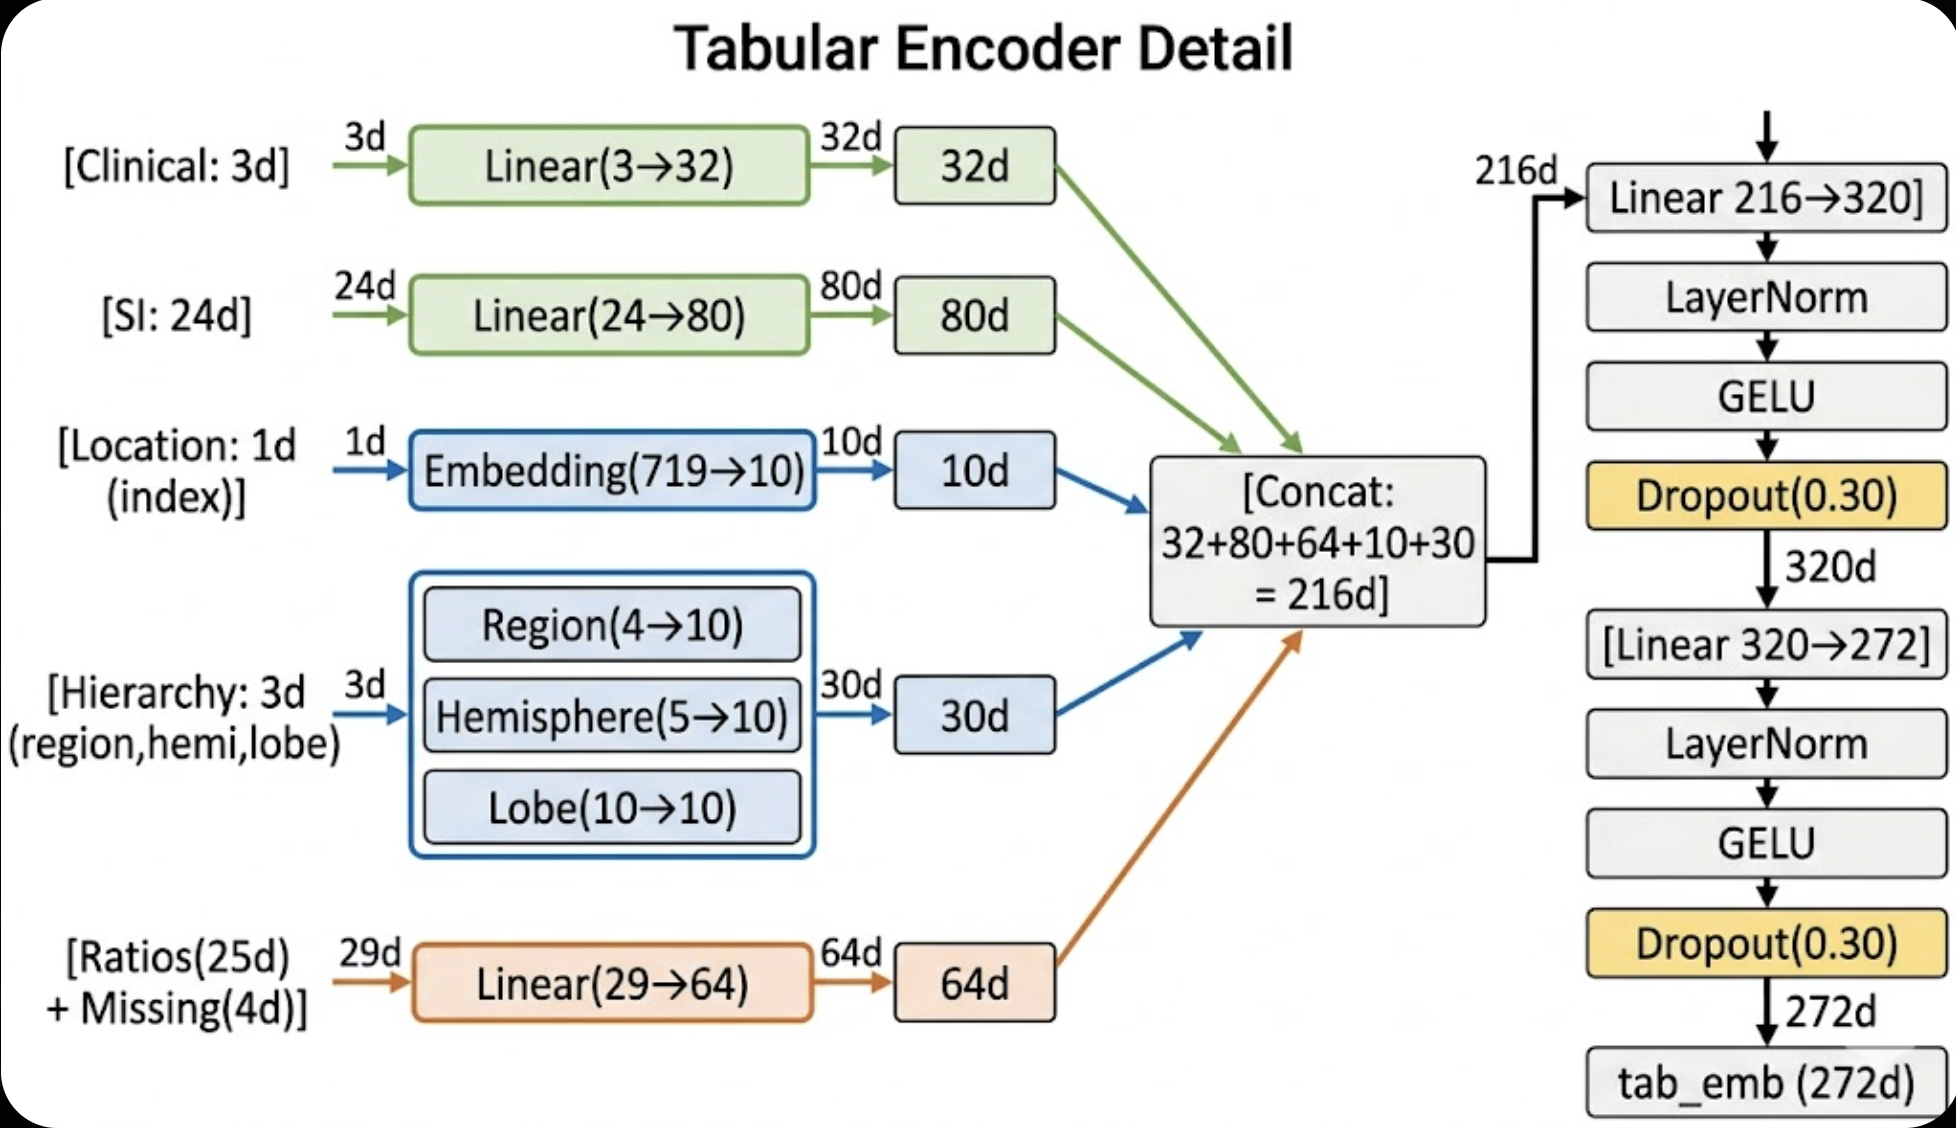
\includegraphics[width=0.85\textwidth]{figures/tabular_encoder.png}
\caption{Tabular encoder. Five feature groups are encoded separately then concatenated and passed through an MLP. Location uses both a learned embedding and hierarchical anatomical parsing.}
\label{fig:tabular_encoder}
\end{figure}

The tabular encoder (Figure~\ref{fig:tabular_encoder}) maps heterogeneous features into a unified 272d embedding. Each feature group gets its own projection before concatenation. This per-group encoding lets the model learn appropriate representations for each data type (binary SI patterns vs.\ continuous ratios vs.\ categorical location). The dropout is 0.30---higher than the report path (0.15) because tabular features are noisier and less structured than text.

\subsubsection{Cross-Modal Gate}

\begin{figure}[H]
\centering
% FIGURE: Cross-Modal Gate Detail
% Generate: figures/cross_modal_gate.png
%
% Layout: Two horizontal paths with a gate mechanism between them
%
% Top path (report):
%   report_emb (288d) → fork:
%     → r_key = Linear(288→64)  ──→  multiply (r_key * t_key) → Linear(64→1) → Sigmoid → g (scalar)
%     → t2r = Linear(272→288)(tab_emb)  ──→  g * t2r  ──→  + report_emb → LayerNorm → report_gated (288d)
%
% Bottom path (tabular):
%   tab_emb (272d) → fork:
%     → t_key = Linear(272→64)  ──→  (shared g from above)
%     → r2t = Linear(288→272)(report_emb)  ──→  g * r2t  ──→  + tab_emb → LayerNorm → tab_gated (272d)
%
% Key elements to highlight:
%   - The single shared gate g (show as a circle with σ, one value in (0,1))
%   - g connects to BOTH paths (show this clearly with arrows)
%   - Label the gate: "g = σ(r_key · t_key)"
%   - Show that g is a SCALAR (not vector) — annotate "g ∈ (0,1)"
%   - When g≈0: paths stay independent (report-only)
%   - When g≈1: paths exchange information (cross-modal)
%
% Use a small truth-table style annotation:
%   "Clear report → g ≈ 0 → rely on report only"
%   "Ambiguous report → g ≈ 1 → blend with tabular"
%
% Figure size: (12, 6), clean style
%
% Data source: model_final.ipynb Cell 14
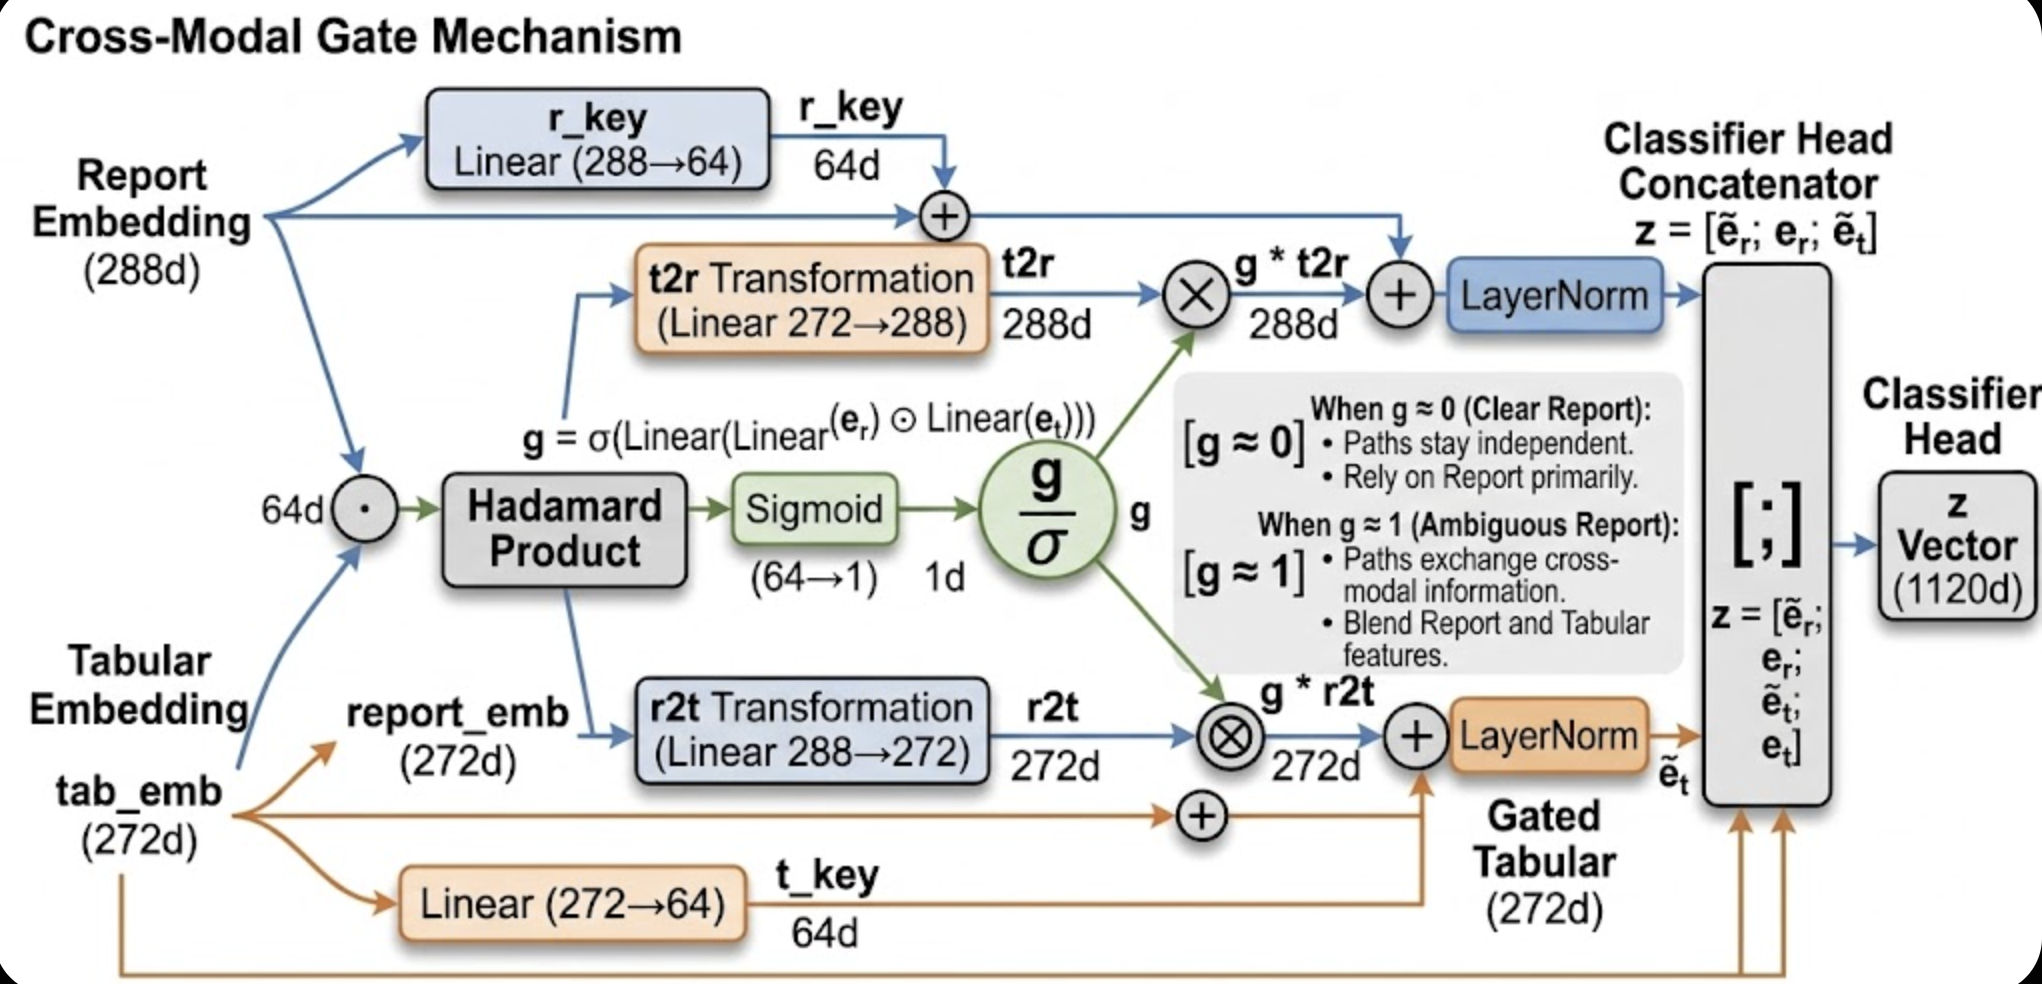
\includegraphics[width=0.9\textwidth]{figures/cross_modal_gate.png}
\caption{Cross-modal gate. A single shared scalar $g$ controls bidirectional information flow between report and tabular paths. When the report is clear, $g \approx 0$ and the model relies solely on the report; when ambiguous, $g$ opens to incorporate tabular evidence.}
\label{fig:cross_modal_gate}
\end{figure}

The cross-modal gate (Figure~\ref{fig:cross_modal_gate}) is the key mechanism. Given report embedding $\mathbf{e}_r$ and tabular embedding $\mathbf{e}_t$, it computes a single shared scalar:

\begin{equation}
g = \sigma\!\big(\text{Linear}(\text{Linear}(\mathbf{e}_r) \odot \text{Linear}(\mathbf{e}_t))\big) \in (0,1)
\end{equation}

This gate controls bidirectional information flow:
\begin{align}
\tilde{\mathbf{e}}_r &= \text{LayerNorm}\big(\mathbf{e}_r + g \cdot \text{Linear}_{t \to r}(\mathbf{e}_t)\big) \\
\tilde{\mathbf{e}}_t &= \text{LayerNorm}\big(\mathbf{e}_t + g \cdot \text{Linear}_{r \to t}(\mathbf{e}_r)\big)
\end{align}

\textbf{Why a single shared gate works:} With only 2K samples, a complex attention mechanism would overfit. The gate has $\sim$25K parameters and learns a simple per-sample decision: trust the report, or supplement with tabular data. The shared gate ensures both paths open or close together, which is easier to learn than independent gates.

\subsubsection{Classifier Head}

The classifier concatenates four components---both gated and original embeddings---as a skip connection:
\begin{equation}
\mathbf{z} = [\tilde{\mathbf{e}}_r;\ \mathbf{e}_r;\ \tilde{\mathbf{e}}_t;\ \mathbf{e}_t] \in \mathbb{R}^{1120}
\end{equation}
This passes through 1120$\to$256$\to$128$\to$5 with LayerNorm, GELU, and decreasing dropout (0.3, 0.2).

\textbf{Why include both gated and original?} The original report embedding is always preserved regardless of gate state. This ensures cross-modal interaction can only help, never hurt---a critical property when 85\% of samples are already well-handled by the report alone.

\subsubsection{Training Configuration}

\begin{table}[H]
\centering
\caption{Neural network training hyperparameters.}
\label{tab:nn_params}
\begin{tabular}{lll}
\toprule
\textbf{Parameter} & \textbf{Value} & \textbf{Why} \\
\midrule
Main learning rate & $3 \times 10^{-5}$ & Standard for fine-tuning \\
BERT LR scale & 0.05 (effective $1.5 \times 10^{-6}$) & Preserve pre-trained weights \\
Fine-tune layers & Top 2 (of 12) & Adapt to tumor terminology \\
Label smoothing & 0.05 & Prevent overconfidence for ensembling \\
Sqrt class weights & $\alpha = 0.5$ & Gentle minority boost \\
Scheduler & Cosine annealing + 3-epoch warmup & Smooth, predictable decay \\
SWA start & 70\% of epochs & Flat minima generalize better \\
Early stopping & Patience 25 & Prevent overfitting \\
Report masking & 12\% of tokens & Don't rely on single keywords \\
Tabular noise & $\sigma = 0.10$ & Robust to measurement shift \\
\bottomrule
\end{tabular}
\end{table}

We train with 5-fold stratified cross-validation (not 10-fold) because 10-fold gives only $\sim$227 validation samples per fold---too few for reliable per-fold evaluation of minority classes. 5-fold gives $\sim$453 validation samples per fold and $\sim$1,813 training samples per fold.

\subsection{Gradient-Boosted Tree Models}
\label{sec:tree}

We train three categories of tree models on different feature sets:

\textbf{MLU (Multi-Model Lineup):} Three models (XGBoost, LightGBM, CatBoost) on the same features: TF-IDF+SVD report (256d) + Clinical+SI (27d) + Location hierarchy (3d) + Cross-modal Ratios (25d) + SI Unknown ratio (1d) = 312d total. Using three algorithms provides diversity through different split-finding strategies. All use 5-fold OOF.

\textbf{NNXGB:} XGBoost on the 5-dimensional OOF probability outputs from the neural network. Here the NN serves as a learned feature encoder: it maps raw reports and tabular data into a 5-d probability vector that captures the NN's uncertainty pattern across classes. The XGBoost then learns non-linear corrections to NN errors (e.g., ``when NN is uncertain between Glioma and Meningioma, default to the larger class''). This two-stage design effectively gives the tree model access to BERT's semantic representations without requiring it to process text directly.

\textbf{ImgTab:} XGBoost on image PCA features (512d) + tabular features ($\sim$57d). Despite low OOF (69.77\%), it makes different errors than text-based models, providing ensemble diversity.

\subsection{Ensemble Strategy}
\label{sec:ensemble}

The final prediction is a weighted average of 6 model probabilities:
\begin{equation}
P(y \mid \mathbf{x}) = \sum_{m=1}^{6} w_m \cdot P_m(y \mid \mathbf{x}), \quad \sum_{m} w_m = 1
\end{equation}

Weights are determined by grid search on OOF predictions (coarse step 0.1, fine step 0.05), optimizing Micro-F1.

\begin{table}[H]
\centering
\caption{Ensemble model weights and individual OOF scores (from 5-fold cross-validation). NN receives 40\% weight due to its complementary error pattern on minority classes, despite lower OOF than tree models.}
\label{tab:ensemble}
\begin{tabular}{lrr}
\toprule
\textbf{Model} & \textbf{Weight} & \textbf{OOF Micro-F1} \\
\midrule
NN (BERT dual-path) & 40\% & 82.35\% \\
MLU\_XGB & 30\% & 86.28\% \\
MLU\_LGB & 30\% & 85.97\% \\
MLU\_CB & 0\% & 85.70\% \\
NNXGB & 5\% & 79.08\% \\
ImgTab & 5\% & 69.77\% \\
\midrule
\textbf{Ensemble} & \textbf{100\%} & \best{87.25\%} \\
\bottomrule
\end{tabular}
\end{table}

\textbf{Why does the NN get 40\% weight despite lower OOF?} Grid search found NN=40\% as OOF-optimal. This reflects the NN's complementary error pattern: it captures minority classes (Pineal/CP 46.15\% vs trees 19--27\%) that tree models miss. The NN uses BERT embeddings that represent semantic meaning rather than surface statistics, which may also be more stable if deployment distributions differ from training (Section~\ref{sec:shift}).
